%!TeX spellcheck = en-US

%\chapter{Open-set and Closed-Set Classification for WGI}
\chapter{Open-set WGI algorithms}

\label{chap:openset}

%----------------------------------------------------------------------------------------

% Define some commands to keep the formatting separated from the content
\newcommand{\keyword}[1]{\textbf{#1}}
\newcommand{\tabhead}[1]{\textbf{#1}}
\newcommand{\code}[1]{\texttt{#1}}
\newcommand{\file}[1]{\texttt{\bfseries#1}}
\newcommand{\option}[1]{\texttt{\itshape#1}}

%----------------------------------------------------------------------------------------

\section{Introduction}\label{chap:openset:sec:intro}

WGI is a task that can be approached either as a closed-set or an open-set classification problem. The former case assumes that there is a well-defined genre palette that covers all possible genres that can be found in our domain. In addition, for each such genre there are representative instances of web-pages to be used as training data. These assumptions are far from realistic in most WGI applications. As already explained in previous chapters, it is not feasible to define a complete genre palette for the Web since there is no consensus over genre labels and new genres are emerging or existing genres evolve through time. On the other hand, it is possible to determine certain web genres where there is general agreement about their characteristics (e.g., blogs, e-shops). For such web genres it is relatively easy to find representative training data. 

Open-set classification is, therefore, a more realistic option to model the WGI task. In this setup, a genre palette covering very specific web genres is given and all other genres are considered as \textit{noise} (i.e., instances of noise should not be assigned to any of the known genres). An effective open-set WGI approach can suit any type of relevant application since it provides the ability to recognize the known web genres without being confused by the presence of noise. It should be underlined that it is expected for noise to outnumber the training instances of the known genres. Web is chaotic and of huge scale and known genres only cover a small part of it.

Open-set classifiers have to deal with an important difficulty: the \textit{Open Space Risk} (OSR). This corresponds to the instance space that lies away from the instances of known genres and can be occupied by samples of an unknown genre. The open-set classifier should be able to set the boundaries of known genres so that to avoid the risk of including an area where an unknown genre is found. This is especially challenging when the dimensionality of the representation is high. This is exactly the case with most of the popular text representation schemes that are composed of hundreds or thousands of features (e.g., character n-grams, word n-grams). It is therefore necessary to perform some kind of feature selection or to use low-dimensional feature space (e.g., word/document embeddings). 

In this chapter, it is introduced and described in detail three open-set WGI methods. The first method is based on one-class classification where only positive examples are considered for each known genre. This does not mean that it is not possible to find negative examples. However, the negative class is too huge and heterogeneous that is quite challenging to extract representative negative samples. The second approach considers training samples for all available known genres and attempts to reduce the effect of high dimensionality of representation by performing repetitive subspacing. The main idea is to build an ensemble of classifiers, each one using a subset of the initial features. The third approach is an extension of the nearest-neighbor classification algorithm and attempts to directly regularize the effect of OSR.

%Finally, all three algorithms have been developed with Noise handling and Outages tolerance in mind. Specifically, all three algorithm can be tuned to regulate their Noise filtering ability with an explicit or implicit threshold. The Noise as explained earlier can be structured or unstructured, i.e. when the noise samples are balanced or not in respect of the genre tags. Note that the noise-filtering regularization threshold is automatically defined for NNDR while training using the OSR as a measure.

In the rest of this chapter, firstly it is described the main properties of open-class classification and discuss main existing approaches. Then, each one of the three proposed methods is analytically presented. 

\section{Open-set Classification}

An open-class classification task is a tuple $(\mathcal{C},\mathcal{K},\mathcal{U})$, where $\mathcal{C}$ is a set of predefined known classes, $\mathcal{K}$ is a set of training samples for the known classes (i.e., for each $c \in \mathcal{C}$ there is a set of training samples $K_c \subset \mathcal{K}$), and $\mathcal{U}$ is a set of unknown samples to be assigned to classes. Each $u \in \mathcal{U}$ may belong to either one $c \in \mathcal{C}$ or none of them. Furthermore, the subset of $\mathcal{U}$ not belonging to any of the known classes is called noise $\mathcal{N}$.  

\subsection{Noise in Open-set Recognition}
\label{chap:openset:sec:Noise_definition}

The previous definition of open-set classification task only considers two kinds of classes, known and unknown. A more detailed analysis is provided in \parencite{geng2018recent}:

\begin{itemize}
    \item \textit{Known-known classes} are the classes for which positive samples are available. This is directly comparable to $\mathcal{C}$.
    \item \textit{Known-unknown classes} consist of negative samples that can be merged into one big artificial class, like background classes \parencite{Dhamija:2018}.
    \item \textit{Unknown-known classes} are classes that can be described using some kind of side-information (e.g., a semantic description). However, there is lack of positive training examples for these classes. The recognition of such classes can be performed by \tetit{zero-shot learning} \parencite{palatucci2009zero}.
    \item \textit{Unknown-unknown classes} are classes without any positive training examples and without any side-information. This directly corresponds to $\mathcal{N}$. 
\end{itemize}

In this thesis we distinguish noise into unstructured and structured forms:

\begin{itemize}
    \item \textit{Unstructured Noise} corresponds to the case there is not a distinction between the unknown classes. In other words, all unknown classes are merged into a single super-class. This is very realistic in WGI applications where it is quite unclear how to define the genre of a large number of web-pages.
    \item \textit{Structured Noise} is composed of distinct unknown classes, that is we consider that each $n \in \mathcal{N}$ belongs to a class $c \notin \mathcal{C}$. Certainly, this information is not given to the open-set classifier but it is only used to estimate its performance. This is also realistic in certain WGI applications where we are interested about the recognition of specific genres and it is also known that several other genres exist.
\end{itemize}

\subsection{The Open-Space Risk}
\label{chap:openset:sec:open_space_risk}

One possibility to build classifiers that can leave some (test) instances unclassified is to introduce a reject option to closed-set classification algorithms. First, a regular closed-set classifier is trained using $\mathcal{K}$. Then, a reject criterion is determined, usually associated with the confidence of the predictions, and each test instance that does not satisfy this criterion is not classified to any of the classes in $\mathcal{C}$ \parencite{onan2018ensemble}. For example, the reject criterion could relate to the difference of probabilities assigned to the two most likely classes in $\mathcal{C}$. If this difference is large, then it is an indication that the instance in question really belongs to the most likely class (the confidence of prediction is high). If, on the other hand, the difference is small (i.e., the confidence of the prediction is low), then this means that the instance most probably does not belong to these classes. 

One big problem of this approach is that it provides strong predictions for the entire instance space. Actually, closed-set classifiers segment the instance space so that instances belonging to the known classes to be well separated. However, this also means that if an unknown class lies in the space that is far away from the known classes, it cannot be easily distinguished anymore. Figure \ref{chap:openset:fig:closed_set_classification}(a) depicts the case where a closed-set classifier is trained to recognize two known classes. Note that the decision boundary affects the entire instance space. There is also an unknown class that lies away from the known classes, almost equally away from both of them, and also near the decision boundary. This scenario can be handled by a rejection option since all members of the unknown class will be equally likely to belong to either of the known classes and, therefore, can be rejected. Figure \ref{chap:openset:fig:open_set_classification}(b) shows a similar case with two known classes and one unknown class. However, this time the unknown class lies deep in the space that belongs to one of the known classes. The member of unknown class are still far away from both known classes but now the rejection option will not work since it seems that one of the known classes is far more likely than the other. 

\begin{figure}[t]
	\begin{center}
    	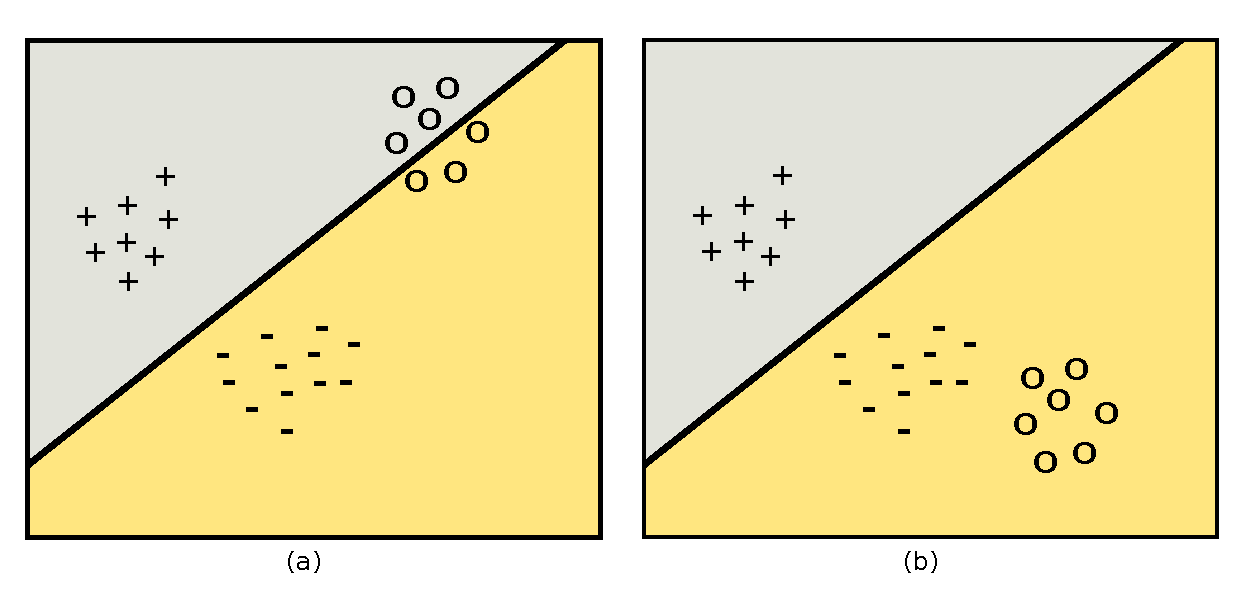
\includegraphics[scale=0.70]{Figures/closed-set_classification_schema.eps}
		\caption{Closed-set classification paradigm. The 'o' samples random unknown for the classification algorithm. The (a) is showing a case where the unknown samples are affecting both prediction for, classes '+' and '-'. The (b) is showing a case where only the '-' prediction is affected}
		\label{chap:openset:fig:closed_set_classification}
	\end{center}
\end{figure}


\begin{figure}[t]
	\begin{center}
    	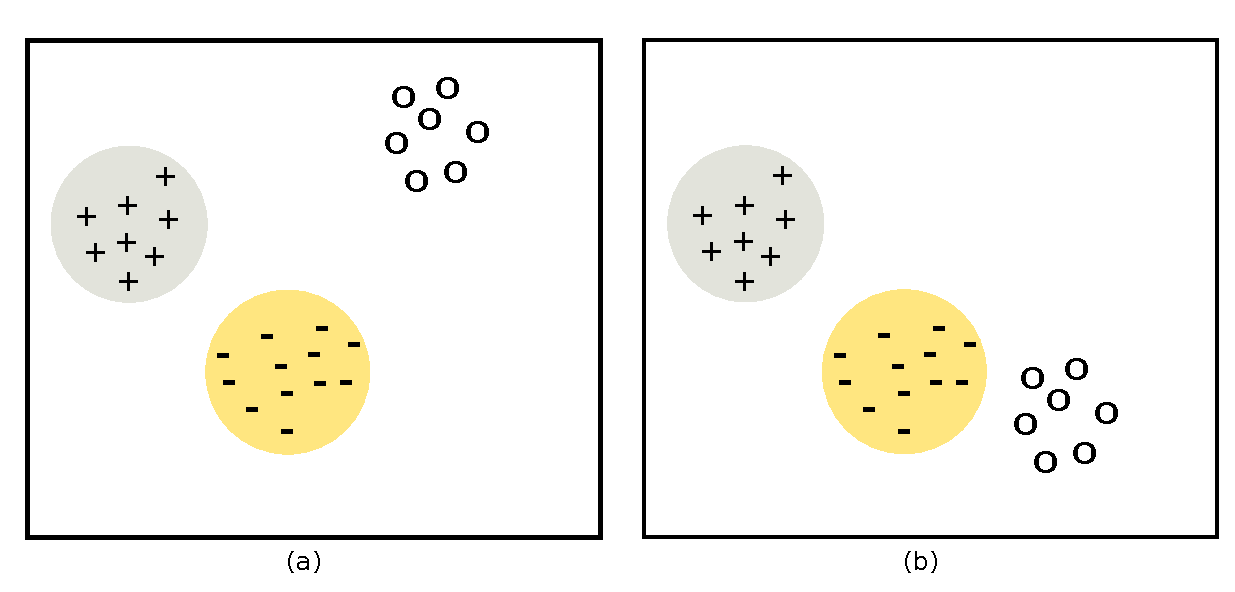
\includegraphics[scale=0.70]{Figures/open-set_classification_schema.eps}
		\caption{Open-set classification paradigm. The 'o' samples random unknown for the classification algorithm. The (a) and (b) are equal to the ones of figure's \ref{chap:openset:fig:closed_set_classification} where in both cases the unknown samples are not affecting the classification performance. However, the model is very conservative. The white area in both cased is the open space, on the contrary to the closed-set classification where the total space is considered part of the red or blue class.}
		\label{chap:openset:fig:open_set_classification}
	\end{center}
\end{figure}

A pure open-set classifier attempts to determine the space that surely belongs to the positive examples of each known class. An example is demonstrated in Figure \ref{chap:openset:fig:open_set_classification} where, similar to the previous case, there are two known classes and one unknown class. However, this time the relative position of the space occupied by the unknown class with respect to the position of the known classes is not important anymore. Note that the most important issue about an open-set classifier seems to be the appropriate definition of the known class boundaries. If the classifier is too conservative, then the space allocated to the known class will be too small and it is possible to exclude some of its members. On the other hand, if the classifier is optimistic, then the area allocated to the known class will be large including neighboring areas of the known class training instances. This is demonstrated in Figure \ref{chap:openset:fig:open_space_risk_schema}. The more optimistic an open-set classifier is the more likely to suffer by the open space risk.

\begin{figure}[t]
	\begin{center}
    	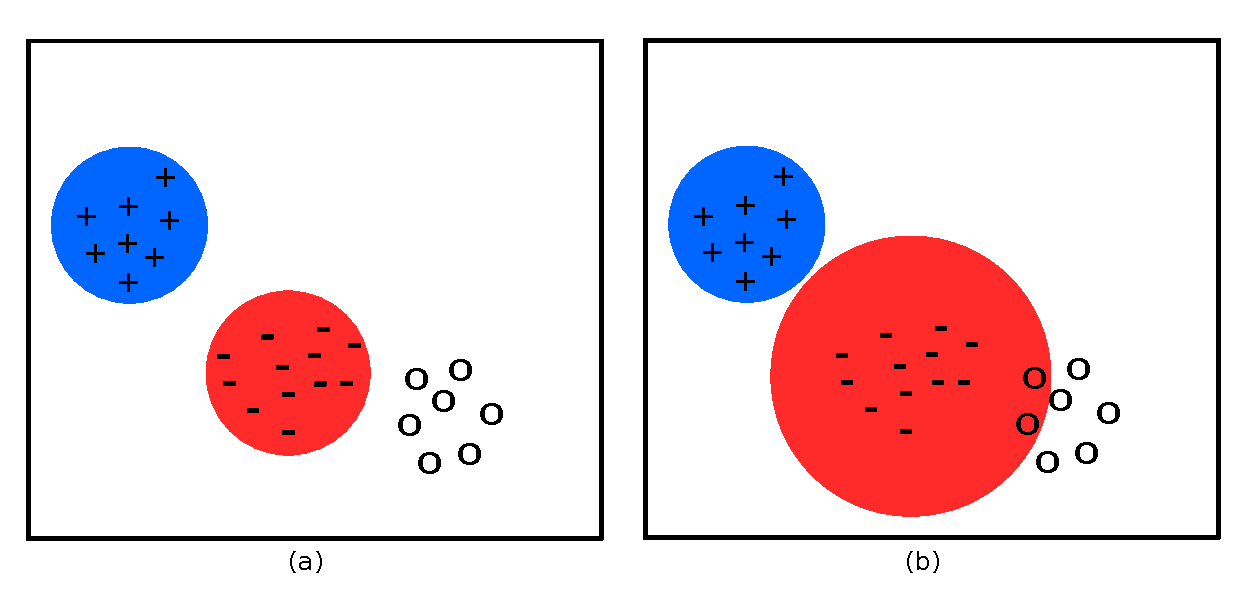
\includegraphics[scale=0.70]{Figures/open_space_risk_schema.eps}
		\caption{Open-set classification paradigm with different \textit{Open Space Risk}. Similarity case of figure \ref{chap:openset:fig:open_set_classification}. The red algorithm in (a) which is \textit{conservative} can be replaced with the green \textit{optimistic} algorithm in (b). However, the optimistic algorithm (b) is more sensitive to the open space risk.}
		\label{chap:openset:fig:open_space_risk_schema}
	\end{center}
\end{figure}


Let $f_y$ be a recognition function for a known class $y$, $f_y(x)=1$ corresponds to the case $x$ is assigned to class $y$ while $f_y(x)=0$ means that $x$ is not recognized to belong to $y$. Then, the open space risk is formally defined as follows \parencite{scheirer2013toward}:

\begin{equation}\label{chap:eval_methods:eq:the_original_open_space_risk}
	R_{o}(f_y) = \frac{\int_{o} f_y(x) dx}{\int_{S_{o}}  f(x_y) dx}
\end{equation}

\noindent
where $O$ corresponds to the positively labeled open space and $S_O$ is the overall positively labeled space including the space of training samples of the known class. The larger the open space risk, the more optimistic the classifier, and the larger area is assigned to the known class.  

An alternative way to define open space is provided in  \parencite{fei2016breaking}. Let $S_O$ be a large sphere of radius $r_O$ including all positive instances of a known class and the positively labeled open space and $B_{r_y}$ be a sphere of radius $r_y$ that ideally includes all positive training examples of known class $y$. Both $S_O$ and $B_{r_y}$ have the same center $cen_y$, the center of positive training instances of class $y$. Then, of to method to constrain the problem is by using the center of the positively labeled training data and defining a radios $r_{o}$ where it will reduce the open space area based on the positively labeled empirically observations. Then the open space $O$ is defined as follows:

\begin{equation}\label{chap:eval_methods:eq:openspace_spherical_constrained}
	O = S_{o} - B_{r_{y}}(cen_{y})
\end{equation}

Given this formulation, where the open space is considered as a bounded spherical area, the main issue in open-set recognition is to appropriately define radius $r_O$ for each known class.

A more formal definition of open-set classification directly involves the open space risk. Let $R_{O}$ be the open space risk and $R_{\epsilon}$ the empirical risk (i.e., the loss function in the training set). Then the objective of open-set classification is to find a function $f$ which minimizes the following \textit{open-set risk}: 

\begin{equation}
\label{eq:open_space_risk}
\argminA_{f} \{R_{O}(f ) + \lambda R_{\epsilon}(f (\mathcal{K}))\}
\end{equation}

\noindent where $f (x) > 0$ implies correct recognition and $\lambda$ is a regularization constant. Thus, open-set risk balances the empirical risk and the open space risk \parencite{geng2018recent}. 

\section{Open-set Classification Paradigms}
\label{chap:openset:sec:Open_Set_Classification_Paradigms}

In the relevant literature, a variety of approaches to open-set recognition can be found. A thorough recent review is provided in \parencite{geng2018recent}. In general, the following main paradigms are usually followed:

\begin{itemize}
    \item One-class classification methods
    \item Modification of traditional ML methods
    \item Deep learning methods
    \item Generative models
\end{itemize}

One way to approach open-set classification is to apply \textit{One-Class classification} (OCC) methods. An OCC method is based on only positive samples of a given class. It is assumed that negative samples are either difficult to obtain or the negative class is so heterogeneous that it not easy to sample it. There are several approaches towards the solution of this problem. A compact survey on OCC is provided in \parencite{khan2010survey}. 

The \textit{Rocchio's algorithm} is the simplest one-class classification algorithm where it has been used for information retrieval tasks because of its simplicity and consistency \parencite{joachims1997probabilistic}. The learning process is just the summation of all the sample vectors of a given class, i.e the \textit{prototype vector}. Then, an arbitrary vector is classified as positive or negative using the angular distance from the prototype vector.

Datta (cited in \parencite{manevitz2002one}) proposed a Naive Bayes Classifier modification for OCC problems and use only positive samples in the learning process. A probability density function of a class $E$ is induced as prediction model. Classifying the a document $d$ involves calculating the probability of the document $p(d|E)$ which is equal to the product of its features $w_{n}$ probabilities $p(w|E)$, where $n$ is the number of document's feature vector. To decide weather the document is classified as positive, a threshold is required to be defined. 

Perhaps the most popular OCC approach is described in \parencite{scholkopf1999estimating}. It is actually a modification of the well-known SVM algorithm to the problem of the overlapping samples distributions, known as $\nu$-SVM \parencite{bishop2006}. The nature of $\nu$-SVM allows to use it in binary classification problems as long as to OCC problems. The parameter $\nu$ is both controlling the fraction of support vectors and the margin errors, i.e. positive samples considered as outliers. The optimization process begins with considering the origin as the only negative example. More details this approach are given in the section \ref{chap:openset:sec:OCSVM_description}.

Outlier-SVM is another SVM-based algorithm introduced in \parencite{manevitz2002one,khan2010survey}. The performance of this model was competitive but not top performer when compared with methods such as One Class Neural Networks, One Class Naive Bayes Classifier, One Class Nearest Neighbor, and Rocchio Prototype. In addition this algorithm is sensitive to the term weighting schema, i.e. \textit{Binary, TF, TF-IDF, etc.}, and vector dimensionality. 

There are, also, some OCC methods exploiting the availability of unlabeled data. \parencite{yu2005single} proposed two OCC algorithms that use positive and unlabeled data for building a classification model that describes the single class boundary. The \textit{Mapping Convergence}(MC) algorithm is incrementally labeling negative data from the unlabeled data set using the margin maximization property of SVM. The \textit{Support Vector Mapping Convergence} (SVMC) optimizes the MC algorithm for fast training. Both algorithms had been compared into real world  classification tasks, letter recognition, and diagnosis of breast cancer with higher performance than \textit{Spy Expectation Maximization} (S-EM), SVM-NN (i.e. C-SVM using unlabeled data point as negative ones) and Naive Bayes Classifier with noise samples \parencite{liu2002partially, li2003learning}.

In contrast to OCC, the majority of the approaches to open-set recognition are able to handle poth positive and negative samples of a given class. Several variations of well-known classification algorithms have been proposed so far. The \textit{1-vs-Set SVM} algorithm introduced in \parencite{scheirer2013toward} was the first attempt to regulate the open space based on formula \ref{eq:open_space_risk} using a second hyperplane parallel to the separating hyperplane. However, the space corresponding to each known class remains unbounded. This means that the open space risk still remains. Another SVM-based approach (W-SVM) consists of two models, a one-class SVM and a binary SVM using a Wibull cumulative distribution function \parencite{scheirer2014probability}. Yet another idea used in the POS-SVM method \parencite{scherreik2016open} models open space risk and empirical risk probabilistically. 

The \textit{Distance Based} algorithms can be adopted in the open-set framework by bounding the true positive samples by the outliers. Nearest Non-Outlier (NNO) algorithms is a center based method where the OSR regularization is their method for keeping the outliers bounded. There are several center based algorithms one of them is the RFSE algorithm developed for this thesis and described in \ref{chap:openset:sec:RFSE_Description}. 

%The Nearest Neighbor algorithm which is also distance based has been adopted to the open-set framework named \textit{Nearest Neighbor Distance Ration (NNDR}). However, this algorithm it is a multi-class classification algorithm and there is no need for an adaption for this as in the above class identification cases.

%The NNDR is using he distance ration in order to regulate both the outlier bound and the OSR. Details for the NNDR are described in section \ref{chap:openset:sec:NNDR_Description} and particularly a special version of it for the WGI task developed for this thesis. It should be noted that due to its decision process where two candidate samples are selected in each step this algorithm is sensitive to outlier, however, it seems that the dimensionality of the feature space can radically change its performance as shown in chapter \ref{chap:word_embeddings}.

%The NNDR is also designed to regulate the OSR and this is part of its learning process where it divided the training data in to segments for regulating this problem in advanced. 

Deep Neural Networks are usually developed with a \textit{SoftMax} function forcing the whole modeling setup to follow a closed-set assumption. However, there have been several efforts where to modify deep learning models for open-set classification, notably using \textit{OpenMax} \parencite{bendale2016towards,cardoso2017weightless}. First, a normal SoftMax model is trained. Then, the layers of the network are modified to be able to recognize (pseudo) unknown classes. Another approach is to follow the adversarial learning setup where it is attempted to generate the unknown classes. One such method, the Generative OpenMax algorithm \parencite{ge2017generative} estimates the decision boundary between known classes and the generated unknown ones.

%The \textit{Extreme Value Theory (EVT)} and \textit{Sparse Representation based} approached is an other group of ML algorithms adopted for the open-set scenario. EVT is a statistical method where the tails of the \textit{distance distributions} can be modeled using the \textit{asymptotic theory}. Thus, the distribution of the \textit{margin distance of each sample to each class} can be approximated. Then this distribution is the boundary for discarding the outlier and the rest of the unknown space (and ultimately the the open space).

%In all the open-set algorithms discussed so far and implemented of this thesis, the goal is the discovery of the threshold implicitly or explicitly, as a rejection criterion in the classification process. Thus the threshold plays a key role. Introducing threshold inevitably the OSR is introduced. An other approach for tackling this problem is the \textit{Dirichlet Process} for the open-set scenario \parencite{geng2018recent}.

Another generative approach is based on the \textit{Dirichlet Process}, a distribution over distributions. This model is not overly depended on the training samples and can adapt to changes in data distribution. The collective decision-based OSR (CD-OSR) method applies co-clustering to model each known class \parencite{geng2018collective}. Each known class can be represented by several of the obtained clusters while some clusters are not associated with any of the known classes. In the testing phase, each instance that falls into these unassociated clusters is assigned to the unknown classes. The main advantage of this generative approach over discriminative-based ones is that it does not need any threshold definition.

\section{Open-set Classifiers for WGI}
\label{chap:openset:sec:Open_set_classifiers_for_WGI}

\subsection{One-Class SVM}\label{chap:openset:sec:OCSVM_description}

The first open-set WGI method introduced in this thesis follows the OCC paradigm. Basically, the main idea is to build a one-class SVM classifier for each class $c \in \mathcal{C}$ using only the positive instances of that class. Ideally, the members of unknonwn classes will not be recognized by any of these one-class classifiers.

One-class SVM attempts to find the contour prescribing the positive samples of the target class. A modification of the traditional SVM algorithm, $\nu$-SVM was introduced in \parencite{scholkopf1999estimating}. Following the logic from the conventional SVM, thoroughly analyzed in \parencite{bishop2006}, the Lagrange multipliers are acquired for solving the optimization problem of formula \ref{chap:openset:sec:eq:3} under constraints described in formulas \ref{chap:openset:sec:eq:4} and \ref{chap:openset:sec:eq:5}. The solution derived is described in formula \ref{chap:openset:sec:eq:12}, i.e. a Lagrangian function that can be used to recognize members of the target class.

\begin{equation}\label{chap:openset:sec:eq:3}
	arg\min_{w,b}\left\{ \frac{1}{\nu\lambda}\sum_{n=1}^{N}(\xi_{n}-\rho)+\frac{1}{2}\|w\|^{2}\right\}
\end{equation}

\begin{equation}\label{chap:openset:sec:eq:4}
	0\leqslant a_{n}\leqslant1/N,\qquad n=1,...,N
\end{equation}

\begin{equation}\label{chap:openset:sec:eq:5}
	\nu\leqslant\sum_{n=1}^{N}a_{n}, \qquad \sum_{n=1}^{N}a_{n}t_{n}=0
\end{equation}

\begin{equation}\label{chap:openset:sec:eq:12}
	\widetilde{L}(a)=-\frac{1}{2}\sum_{n=1}^{N}\sum_{m=1}^{M}a_{n}a_{m}t_{n}t_{m}k(x_{n,}x_{m})
\end{equation}

\nointend where $N$ is the size of the positive samples of the target class and $\nu$ a hyper-parameter. The latter has the following properties:

\begin{itemize}
	\item $\nu$ is an upper bound on the fraction of outliers.
	\item $\nu$ is a lower bound on the fraction of support vectors.
	\item $\nu$ values cannot exceed 1.
\end{itemize}

In practice, different values of $\nu$ are defining different proportion of the training sample as outliers. For example in \parencite{scholkopf1999estimating} is showed that in their experiments when using $\nu=0.05$, 1.4\% of the training set has been classified as outliers while using $\nu=0.5$, 47.4\% is classified as outliers and 51.2\% is kept as SVs.

In the prediction phase in order for an OCSVM model to decide whether a document is belonging to the target genre-class (or not) a \textit{decision function} is used. The decision function indicates the distance of the document, positive or negative, to the hyperplane separating the classes. In the case of OCSVM we are usually only interested whether the decision function is positive or negative for deciding if an arbitrary document belonging or not to the target class.

In this thesis the Ensemble form of the OCSVM is used and first proposed in \parencite{pritsos2013open}. The \textit{OCSVM Ensemble} (OCSVME\footnote{The OCSVM ensemble was implemented in Python using the \textit{scikit-learn} package found in http://scikit-learn.org}) is as analytically described in algorithm \ref{chap:openset:sec:alg:OCSVM_Ensemble}. In the case of the OCSVME, we are interested in the positive and negative decision of each ensemble's classifier, and the decision scores.

\hfill

\begin{algorithm}[H][t]
\caption{The \textit{OCSVM} algorithm.}\label{chap:openset:sec:alg:OCSVM_Ensemble}
\KwData{ $G$ a genre palette and $W_{g}$ a set of known web-pages for each $g \in G$,
		 $w$ an unknown webpage of the $W_{a}$ arbitrary webpages set,
		 $F$ the feature set,
		 $\boldsymbol\nu$ the nu hyper-parameter of OCSVM,
         }
\KwResult{ $r \in \{G,\,\emptyset\}$ }
$score[:, :]$=0, the score 2D matrix where rows are for genre's class tags and columns for each webpage under evaluation
\For{each $g \in G$}{
  $Model(g) = ocsvmTrain(W_{g},F,\boldsymbol\nu)$, train a OCSVM model in vector space $F$ with hyper-paramenter $\boldsymbol\nu$ for genre $g$\;
}
\For{each $g \in G$}{
    \For{each $w \in W_{a}$}{
        $score[g, w] = ocsvmApply(Model(g),F,w)$, the distance of the unknown page $w$ from the hyperplane\;
    }
}
\eIf{$max(score[:, :])< 0$}{
    $r \in \emptyset$, i.e. none of the known genres or "I don't know";
}
{
        $r = argmax_{g \in G}(score[:, :])$, i.e. $w$ belongs to the genre of highest score\;
    }
\end{algorithm}

\hfill

In training phase of the ensemble one OCSVM is built for each known genre label. The hyper-parameter $\nu$ has the same value for all OCSVM models. In the prediction phase, the document is assigned to the class with the highest positive distance from the hyperplane (or the contour for OCSVM). If all OCSVMs return a negative distance (i.e. the web-page does not belong to this genre) the document remains unclassified, that is the final answer corresponds to "I Don't Know".


\subsection{Random Feature Subpacing Ensemble}\label{chap:openset:sec:RFSE_Description}

The RFSE algorithm is a variation of the method presented by Koppel et al. \parencite{koppel2011authorship} for the task of \textit{Author Identification}. In the original approach, there is only one training example for each author and a number of simple classifiers is learned based on random feature subspacing. Each classifier uses the \textit{Cosine (or other) distance} to estimate the most likely author. It is more likely for the true author to be selected by the majority of the classifiers since the used subset of features will still be able to reveal that high similarity. That is, the style of the author is captured by many different features so a subset of them will also contain enough stylistic information. Since WGI is also a style-based text categorization task, this idea should also work for it.

\hfill

\begin{algorithm}[H][t]
\caption{The \textit{RFSE} algorithm.}\label{chap:openset:sec:alg:RFS-Ensemble}
\KwData{ $G$ a genre palette and $W_{g}$ a set of known web-pages for each $g \in G$,
		 $w$ an arbitrary web-page of the $W_{a}$ arbitrary webpages set,
		 $F$ the feature set,
		 $fs$ a fraction of feature set size,
		 $I$ a number of iterations,
		 $\boldsymbol\sigma$ the decision threshold }
\KwResult{ $r \in \{G,\,\emptyset\}$ }
\For{each $g \in G$}{
  $centroid[g] = average(W_{g},F)$, average all known web-pages $W_{g}$ of genre $g$ to build a centroid vector\;
  $score[g]=0$\;
}
\Repeat{$I$ times}{
    $f = subset(F,fs)$, Randomly choose $fs$ features from the full feature set $F$\;
    \For{each $g$ in $G$}{
        \For{each $w$ in $W_{a}$}{
    	   $sim[g, w] = similarity(w, centroid(g), f)$, estimate similarity of unknown page $w$ with $centroid(g)$ in vector space $f$\;
        }
    }
   	$maxg = argmax_{g \in G}(sim[:, :])$, find the top match genre\;
   	$score(maxg) = score(maxg) + 1$, increase the score of top match genre\;
}

\eIf{$max(score(g))/I > \boldsymbol\sigma$}{
   $r = argmax_{g \in G}(score(g))$, assign the unknown page to genre with maximum top matches\;
}
{
      $r = \emptyset$, none of the known genres or "I don't know"\;
}
\end{algorithm}

\hfill

In this thesis the RFSE method is adopted, as introduced in \parencite{pritsos2013open} and shown in \textit{Algorithm \ref{chap:openset:sec:alg:RFS-Ensemble}}. There are multiple training examples for each available class. To maintain simplicity of classifiers, we have used a \textit{centroid vector} for each genre. In the training phase, a centroid vector is formed, for every class, by averaging all the Term-Frequency (TF) vectors of the training examples of web pages for each genre.

The class centroids are all formed for a given feature type. Then, an evaluation sample is compared against every centroid and this process is repeated $I$ times. Every time a different feature sub-set is used. Then, the scores are ranked from highest to lowest and we measure the number of times the sample is top-matched with every class. The sample is assigned to the genre with maximum number of matches given that this score exceed a predefined $\sigma$ threshold. In the opposite case, the sample remains unclassified, the RFSE responds "I Don't Know".

With respect to the similarity function, we examine cosine similarity (similar to \parencite{pritsos2013open}) and MinMax similarity (inspired by \parencite{koppel2014determining}). Moreover, measure that combines these two similarity functions, can be used. Then the most confident measure can be used in each iteration. More specifically, since Cosine and MinMax may have different mean and standard deviation for the set of all evaluation samples and all iterations per sample. Note that their values should first be normalized. Then, for each evaluation sample and each iteration we select the one with maximum normalized value. We call this similarity measure \textit{Combo}.

\subsection{Nearest Neighbors Distance Ratio}\label{chap:openset:sec:NNRD_Description}

The \textit{Nearest Neighbors Distance Ratio} (NNRD\footnote{The implementation of the NNRD algorithm can be found at \url{https://github.com/dpritsos/OpenNNDR}, where it is implemented in Python/Cython and can significantly accelerated using as much as possible CPUs due to its capability for concurrent calculations in C level speed. Since, NNRD is a rather slow classification method, we have seen in practice that there is up to 100 time acceleration from the capability to exploit a cloud service with 32 vCPUs (Xeon) compare to 4-core/8-threads i7 CPU.}) algorithm has been proposed as open-set algorithm by \parencite{mendesjunior2016}. In this thesis a specialized version has been implemented for the WGI task. In the original approach euclidean distance has been used because of the variation of data set on which the algorithm has been evaluated. In this thesis cosine distance is used, because in text classification is being confirmed to be the proper choice in hundreds of publications. Moreover, the cosine distance is comparable to the results of the \textit{Random Feature Sub-spacing Ensemble} algorithm found in \parencite{pritsos2018open} and also is tested in the open-set experiments of this thesis found in chapter \ref{chap:noise}.

The NNRD algorithm is an extension of the simple \textit{Nearest Neighbors} NN algorithm where additionally to the sets of training vectors (one set for each class) a threshold is selected by maximizing the \textit{Normalized Accuracy} (NA) as shown in equation\ref{chap:openset:sec:eq:NA}) on the \textit{Known} and the \textit{Marked as Unknown samples}.

\begin{equation} \label{chap:openset:sec:eq:NA}
    NA = \lambda A_{KS} + (1 - \lambda) A_{MUS}
\end{equation}

\noindent
where $A_{KS}$ is the \textit{Known Samples Accuracy} and $A_{MUS}$ is the \textit{Marked as Unknown Samples Accuracy}. The balance parameters $\lambda$ regulates the mistakes trade-off on the known and marked-unknown samples prediction.

The optimally selected threshold is the the \textit{Distance Ratio Threshold} (DRT) where NA is maximized. Equation \ref{eq:DR} is used for calculating the Distance Ratio (DR) of the two nearest class samples, say $s_{c_{a}}$ and $u_{c_{b}}$, to a random sample $r_{x}$ under the constrain $c_{a} \neq c_{b}$, where $c_{g}$ is the sample's class.

It is very important to note that the $c_{g}$ is trained in an open-set framework, therefore, the samples pairs selected for comparison might either be from the known of the marked as unknown samples. Thus $g \in {1,2,...,N}$ and $g = \emptyset$ when samples is marked as unknown.

\begin{equation} \label{eq:DR}
    DR = \frac{D(r_{x}, s_{c_{a}})}{D(r_{x}, s_{c_{b}})}
\end{equation}
\noindent
where $D(x,y)$ is the distance between the samples where in this study is the \textit{Cosine Distance}.

Therefore, the fitting function of the NN algorithm, described in pseudo-code \ref{chap:openset:alg:NNDR_fitting}, is the optimization procedure to find the DRT values for classes respective sets of training samples where NA is maximized.

\hfill

\begin{algorithm}[H][t]
\caption{\textit{Nearest Neighbor Distance Ratio} training data fitting function}\label{chap:openset:alg:NNDR_fitting}
\KwData{$G$ the set of genre class tags $\{1,2,...,N\}$,
        $p$ the hyper-parameter regulates the percentage of $G$ tags will be marked as unknown,
        $k$ the hyper-parameter regulates the percentage of known $G$ tags that will be keept for validation only,
        $T$ the \textit{Distance Ratio} thresholds set than will test for finding the one which is minimizing the \textit{Normalized Accuracy},
        $\lambda$ regulates the mistakes trade-off on the known and marked-unknown samples prediction (see eq.\ref{eq:DR}),
        $C[g]$ the matrix of class vector sets one for every genre class tag $g \in G$}
\KwResult{$DRT$ the \textit{Distance Ration Threshold} calculated by the NNRD algorithm's fitting function, $C[g]$}

$K^{G}_i, K^{G}_{validation}_i, U^{G}_{validation}_i, I^{G} = Split(G,p,k)$ splitting the $G$ tags in to known/unknown samples combinations using the $p$ and $k$ hyper-parameters. The amount of split combinations is calculated by the equations \ref{eq:splt_percent} and \ref{eq:splt}.\;

$V^{G} = U^{G}_{validation} \cup K^{G}_{validation}$ the validation set is the union of the $I$ splits of the known-validation and the marked-as-unknown sets, of the whole training set\;

\For{each $i \in I$}{
    $D^{cos}_{VK}[i] = COS_{D}(V^{G}_i, K^{G}_i)$ calculating all the Cosine Distances between the web-page of $K^{G}$ and $V^{G}$ sets for \textit{every $I$ split combination};
}

$Ci^{min}_{A} = argmin(D^{cos}_{VK})$ getting the indices of the closest classes from $V$\;
$Ci^{min}_{B} = argmin(D^{cos}_{VK})$ getting the indices of the \textit{second closest} classes from $V$\;

$R_{V} = D^{cos}_{VK}[Di^{min}_{A}] / D^{cos}_{VK}[Di^{min}_{B}]$ calculating the Distance Rations $R$ for all the vectors in $V$

$NA^{max} \gets 0$ initializing \textit{Maximized Normalized Accuracy} with $0$ value.
$DRT \gets 0$ initializing \textit{Distance Ratio Threshold} with $0$ value.

\For{each $drt \in T$}{

    \For{each $r, i \in \{R_{V}, count(R_{V})\}$}{

        \eIf{$r < drt$}{
            $vi = Ci^{min}_{A}[i]$ keep the respective index\;
            $Y[i] = G[vi]$ setting the genre's class tag as prediction for this random vector of set $V$\;
        }
        {
            $Y[i] = \emptyset$ setting as none of the known genres or "I don't know"\;
        }

    }

    $NA_{V} = NormalizedAccuracy(Y, R_{V})$ calculating the Normalized Accuracy as shown in equation \ref{eq:NA} for tested threshold $drt$\;

    \eIf{$NA_{V} > NA^{max}$}{
        $NA^{max} \gets NA_{V}$ keeping the maximum $NA$ until the outer for-loop finishes\;
        $DRT \gets drt$ keeping the \textit{Distance Ratio Threshold} maximizes the \textit{Normalized Accuracy}\;
    }

}

\end{algorithm}

\hfill

In the optimization procedure the training samples are split based on their class tags $c_{x}$. Then some class tags are \textit{marked as unknown} and some are left being known. Therefore, all the samples of the marked as unknown are used only in the validation subset while the known class tags samples are farther split into the classes sets (one for each class) and into the known validation set. Then, samples of the validation sets, both then known and then marked as unknown, are used seamlessly for calculating the set of Distance Rations (one for each class). Afterwards, a set of DRT values are tested given a range of values $R \in {t_{1}, t_{2}, t_{n}}$ beforehand where the $t_{x}$ is selected which is maximizing the NA of the validation set.

The splitting procedure the of the training set is regulated by a hyper-parameter $p$ which defines the percentage of the class tags set $g \in {1,2,...,N}$ where they will be marked as unknown. Then the total number of all possible splitting combination are calculated and these split-sets are used for finding the DRT. The combination are found using equations \ref{eq:splt_percent} and \ref{eq:splt}, where eq.\ref{eq:splt} is the \textit{Binomial Coefficient}.

\begin{equation} \label{eq:splt_percent}
    U_{num} = int(N * p)
\end{equation}

\noindent
where $N$ is the size of the class tags set ${1,2,...,N}$ and $p$ is the percentage regulation parameter for keeping the number of tags to be marked as unknown.

\begin{equation} \label{eq:splt}
    S_{num} = \frac{N!}{U_{num}!(N-U_{num})!}
\end{equation}

The NNDR is a open-set classification algorithm, therefore, every random sample will be classified to one of the classes the NNRD has been fitted or to the unknown when its DR is greater then DRT. While training as explained above the DRT values are tested incrementally until the optimal data fitting for the training function.

In prediction phase the DRT is passed to the NNDR prediction function together with the random samples and the training samples as shown in pseudo-code \ref{alg:NNDR_prediction}.

\hfill

\begin{algorithm}[H][t]
\caption{\textit{Nearest Neighbor Distance Ratio} prediction function}\label{alg:NNDR_prediction}
\KwData{ $W$ the vector set of the random web-page to be classified,
         $C[g]$ the matrix of class vector sets one for every genre class tag $g \in G$,
		 $DRT$ the \textit{Distance Ration Threshold} calculated by the NNRD algorithms fitting function}
\KwResult{ $Y \in \{G,\,\emptyset\}$,
           $R$ the Distance Ratio scores vector, one score for every input vector of the random set $W$}

\For{each $g \in G$}{
    $D^{cos}_{C_{g}X} = COS_{D}(C[g], X)$ calculating all the Cosine Distances between the random web-page vectors and the class vectors of class $g$\;
}

$Ci^{min}_{A} = argmin(D^{cos}_{C_{g}W})$ getting the indices of the closest classes from $W$\;
$Ci^{min}_{B} = argmin(D^{cos}_{C_{g}W})$ getting the indices of the \textit{second closest} classes from $W$\;

$R_{W} = D^{cos}_{C_{g}W}[Di^{min}_{A}] / D^{cos}_{C_{g}W}[Di^{min}_{B}]$ calculating the Distance Rations $R$ for each vector $w \in W$

\For{each $r, i \in \{R_{W}, count(R_{W})\}$}{

    \eIf{$r < DRT$}{
        $i_{g} = Ci^{min}_{A}[i]$ keep the respective index\;
        $w_{i} = G[i_{g}]$ setting the genre's class tag as prediction for this web-page $w_{i} \in W$\;
    }
    {
        $w_{i} = \emptyset$ setting as \textit{unknown} (or "I don't know") the class tag of this web-page \;
    }

}

\end{algorithm}

\hfill

\section{Summary}\label{chap:openset:sec:NNRD_Description}

In this section the three implementation of open-set algorithms are presented which they are specialized for the WGI task, however, they can work also in different open-set domains. The definition of the open-set framework in the identification and the multi-class classification, forms.

In the context of the open-set framework and multi-class classification the \textit{Structured and Unstructured Noise} is defined for the first time. These definition are standing on the definition of the four special sample cased in the open-set framework. These definitions are expanding the \textit{Positive} and \textit{negative} categories of the samples found on the closed set scenarios with the \textit{Known} and \textit{Unknown} cases. 

The difference of the One-Class classification (and Novelty Detection) with the Open-set Classification is clarified and defined. Also, the \textit{Openness} of the problem is initially discussed which is indicating the level of difficulty of an open-set problem, where its score measurement method is discussed farther in chapter \ref{chap:eval_methods}.

Finally, the three major issues are captured using these three algorithms developed in this thesis; the luck of negative samples with the OCSVME, the noise tolerance with the RFSE, and the regularization of the open space risk with the NNDR. Although, the last is requiring the \textit{Distributional Features (an Neural Language Modeling)} input, discussed in chapter \ref{chap:word_embeddings}, for satisfying the its requirements of the WGI task.